\documentclass[conf]{new-aiaa}
%\documentclass[journal]{new-aiaa} for journal papers
\usepackage[utf8]{inputenc}

\usepackage{graphicx}
\usepackage{amsmath}
\usepackage[version=4]{mhchem}
\usepackage{listings}
\usepackage{color}
\usepackage{siunitx}
\usepackage{longtable,tabularx}
\usepackage{subcaption}
\usepackage{cleveref}
\usepackage{appendix}
\setlength\LTleft{0pt}

\title{Computing the Mach contour of expansion Corner Supersonic Nozzle by using Method of Characteristic}

\author{Ranjithkumar B}

\definecolor{mygreen}{rgb}{0,0.6,0}
\definecolor{mygray}{rgb}{0.5,0.5,0.5}
\definecolor{mymauve}{rgb}{0.58,0,0.82}

\lstset{
  backgroundcolor=\color{white},   % choose the background color; you must add \usepackage{color} or \usepackage{xcolor}; should come as last argument
  basicstyle=\footnotesize,        % the size of the fonts that are used for the code
  breakatwhitespace=false,         % sets if automatic breaks should only happen at whitespace
  breaklines=true,                 % sets automatic line breaking
  captionpos=b,                    % sets the caption-position to bottom
  commentstyle=\color{mygreen},    % comment style
  deletekeywords={...},            % if you want to delete keywords from the given language
  escapeinside={\%*}{*)},          % if you want to add LaTeX within your code
  extendedchars=true,              % lets you use non-ASCII characters; for 8-bits encodings only, does not work with UTF-8
  firstnumber=0001,                % start line enumeration with line 1000
  frame=single,                    % adds a frame around the code
  keepspaces=true,                 % keeps spaces in text, useful for keeping indentation of code (possibly needs columns=flexible)
  keywordstyle=\color{blue},       % keyword style
  language=Octave,                 % the language of the code
  morekeywords={*,...},            % if you want to add more keywords to the set
  numbers=left,                    % where to put the line-numbers; possible values are (none, left, right)
  numbersep=5pt,                   % how far the line-numbers are from the code
  numberstyle=\tiny\color{mygray}, % the style that is used for the line-numbers
  rulecolor=\color{black},         % if not set, the frame-color may be changed on line-breaks within not-black text (e.g. comments (green here))
  showspaces=false,                % show spaces everywhere adding particular underscores; it overrides 'showstringspaces'
  showstringspaces=false,          % underline spaces within strings only
  showtabs=false,                  % show tabs within strings adding particular underscores
  stepnumber=2,                    % the step between two line-numbers. If it's 1, each line will be numbered
  stringstyle=\color{mymauve},     % string literal style
  tabsize=2,                       % sets default tabsize to 2 spaces
  % title=\lstname                 % show the filename of files included with \lstinputlisting; also try caption instead of title
}

\begin{document}

\maketitle

\section{Problem Definition}

\begin{figure*}[!h]
	\centering
	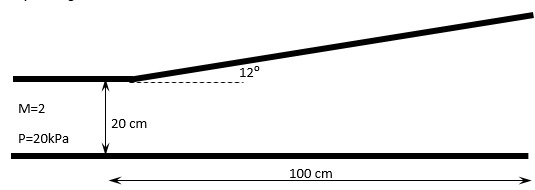
\includegraphics[scale=0.5]{results/question.png}
\end{figure*}

\par The Compression corner has equivalent angle on both sides with inlet Mach number 3.5. The inlet and outlet the flow is turn with respect to the angle of the corner.\\

\textbf{SOLUTION:}\\

\par Given data
\begin{align*}
	M_1 &= 2 \\
	P_1 &= 20 \ kPa \\
	\theta & = 12^0
\end{align*}

\par The solution is done by following procedure\\

\par For the test case, The number of nodes consider as 10 on the wall and 5 on the height, therefore the total number of nodes in this problem is  \\
\begin{align*}
	N_{t} & = N_w^2+(N_i-1)^2
\end{align*}
\par The Top Boundary nodes and the Bottom boundary nodes were calculated by using the bellow formulae, here I is denote for the Each inlet node numbers
\begin{align*}
	btm-wall & = I*(2 \times N(inlet)-1) \\
	top-wall & = btm_wall[previous] + (N -1) \\
\end{align*}

\section{Formula and Procedure}
\subsection{Computing Mach number}
\par The Reimann invarients are calculated by using the inlet data for the inlet Nodes. After computing the inlet Node values depend on the inlet values we can continuously computing the succesive Nodes. The initial \(K_1 \ and \ K_2\) were calculated by intlet angle and the Mach number. \\
\begin{align*}
	K_1 &= \nu + \theta \\
	K_2 &= \nu - \theta
\end{align*}
\par The Reimann invarients won't change until it get hit and refect by the wall or the boundary. Therefore we can compute Prandtl-Meyer expansion function ($\nu$) and the angles ($\theta$) by using Reimann invarients.\\
\begin{align*}
	\nu &= \frac{K_1 + K_2}{2} \\
	\theta &= \frac{K_1 - K_2}{2}
\end{align*}
The Bottom wall have only \(K_1\) and Top wall have only the \(K_2\) and we know the angle of the top and bottom surface. With these information we can calculate P-M function on that Node.
\begin{align*}
	\text{for bottom wall} \\
	\nu &= K_1 - \theta \\
	\text{for top wall}\\
	\nu &= K_2 + \theta
\end{align*}

\par The Mach numbers at each points were calculated by using
Prandtl-Meyer expansion function relation
\begin{align*}
	\nu(M) = \sqrt{\frac{\gamma+1}{\gamma-1}}tan^{-1}\sqrt{\frac{\gamma-1}{\gamma+1}\left(M^2-1\right)} - tan^{-1}\sqrt{M^2-1}
\end{align*}
\par Now we know the Angles and Mach number of each Nodes.\\
\subsection{Computing Location}
\par We know the Mach number of each Nodes, with that value we can calculate the Mach angle ($\mu = \arcsin\frac{1}{M}$). Using Mach angle and the flow angle we can compute the X and Y location. 
\begin{align*}
	S_1 &= \frac{tan(\theta-\mu)_A + tan(\theta-\mu)_B}{2} \\
	S_2 &= \frac{tan(\theta+\mu)_A + tan(\theta+\mu)_B}{2} \\
	y_D &=y_A + (x_D - x_A) S_1 \\
	y_D &=y_B + (x_D - x_B) S_2 \\
	x_D &= \frac{(S_2 x_B - S_1 x_A) + (y_A - y_B)}{S_2-S_1}
\end{align*}
\par Then the Top and Bottom wall Nodes location is calculated by using the slope given bellow.\\
\begin{align*}
	\frac{dy}{dx}_A & =\tan(\theta-\mu)_A \\
	\frac{dy}{dx}_B & =\tan(\theta-\mu)B \\
\end{align*}

\pagebreak
\section{Results:}
\begin{figure*}[!h]
	\centering
	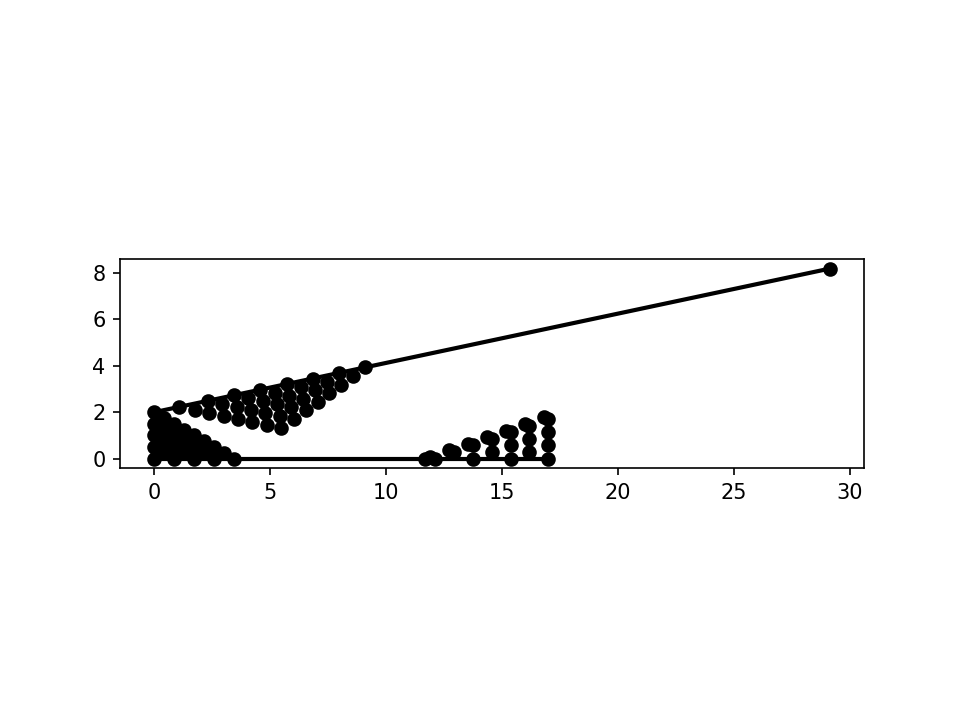
\includegraphics[scale=0.8]{results/Grid.png}
\end{figure*}

\begin{figure*}[!h]
	\centering
	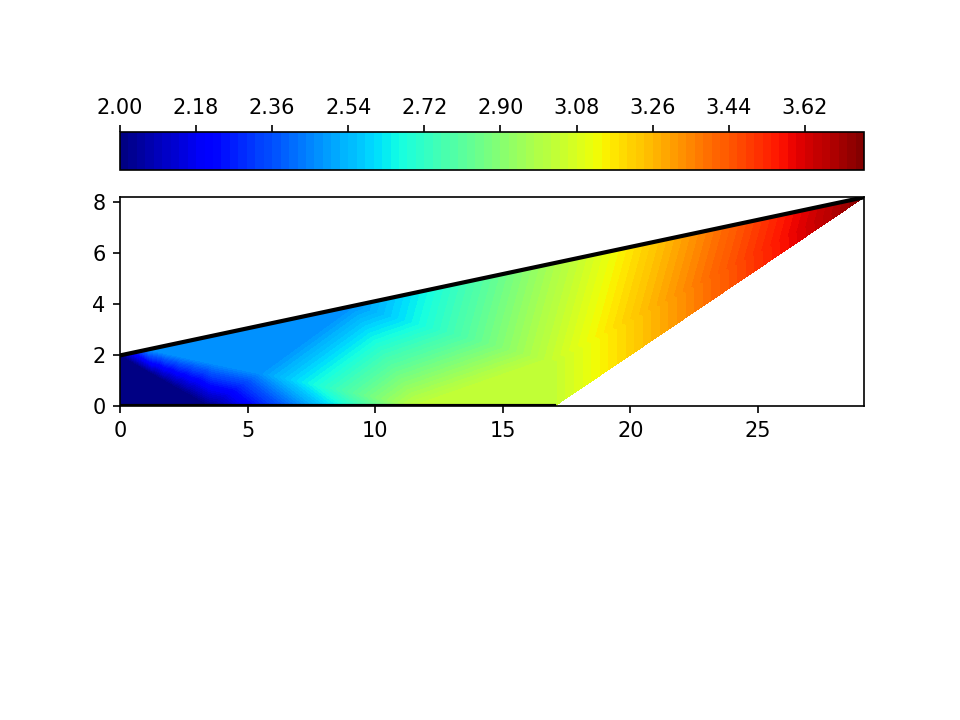
\includegraphics[scale=0.8]{results/Contour.png}
\end{figure*}

\pagebreak

\begin{appendices}
    \section{Appendix - Python code}\label{appendixA}
    \lstinputlisting[language=Python]{results/MOC.py}
\end{appendices}

\end{document}
